\chapter{SIMO and MISO Multi-path}

To avoid unnecessary repetition, we will do what we did in the previous step, except for the implementation on these two systemsز
\section{SIMO}
\begin{figure}[!h]
	\centering
	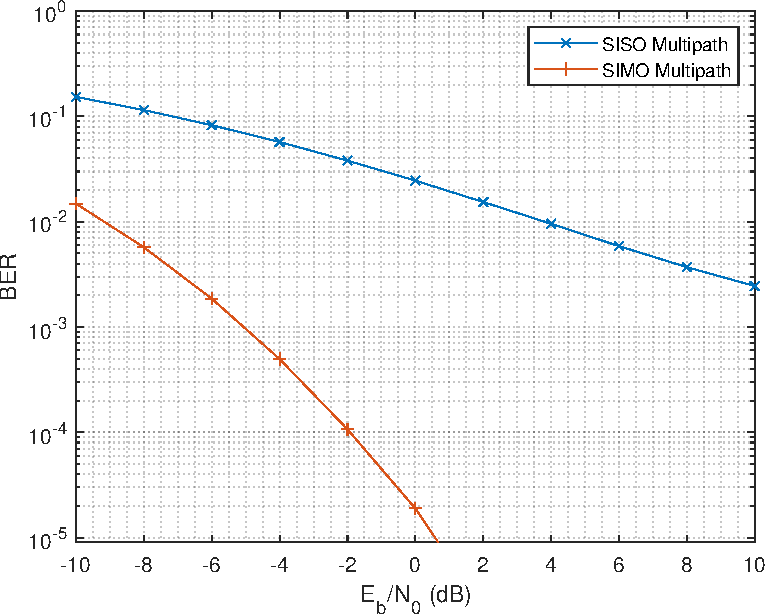
\includegraphics[width=1\linewidth]{figures/SISO_SIMO Multipath.pdf}
	\caption{SISO LOC vs Multi-path}
	\label{32545}
\end{figure}
as we can see in Figure[\ref{32545}], for multi-path SIMO, the BER is smaller than multi-path SIMO , and that's because of the spatial diversity and also because the signal is forming in a beam that is more focusing in one direction.
\section{MISO}
\begin{figure}[!h]
	\centering
	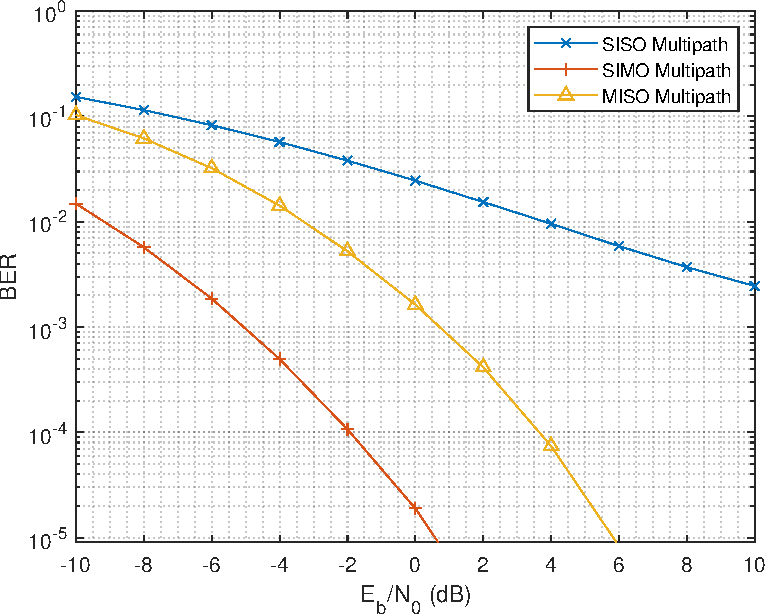
\includegraphics[width=1\linewidth]{figures/SISO_SIMO_MISO Multipath.pdf}
	\caption{SISO LOC vs Multi-path}
	\label{3575}
\end{figure}

and for multi-path MISO, the antenna in the \Tx is less directed towards the \Rx than the \Rx was in the SIMO system, the beam is less saturated and the destructive fading is more than it was in this case at the \Rx, so we are seeing a better BER for SIMO here Figure[\ref{3575}].

\newgeometry{margin=0pt}
\newpage
\vfill
\begin{figure}
	\centering
	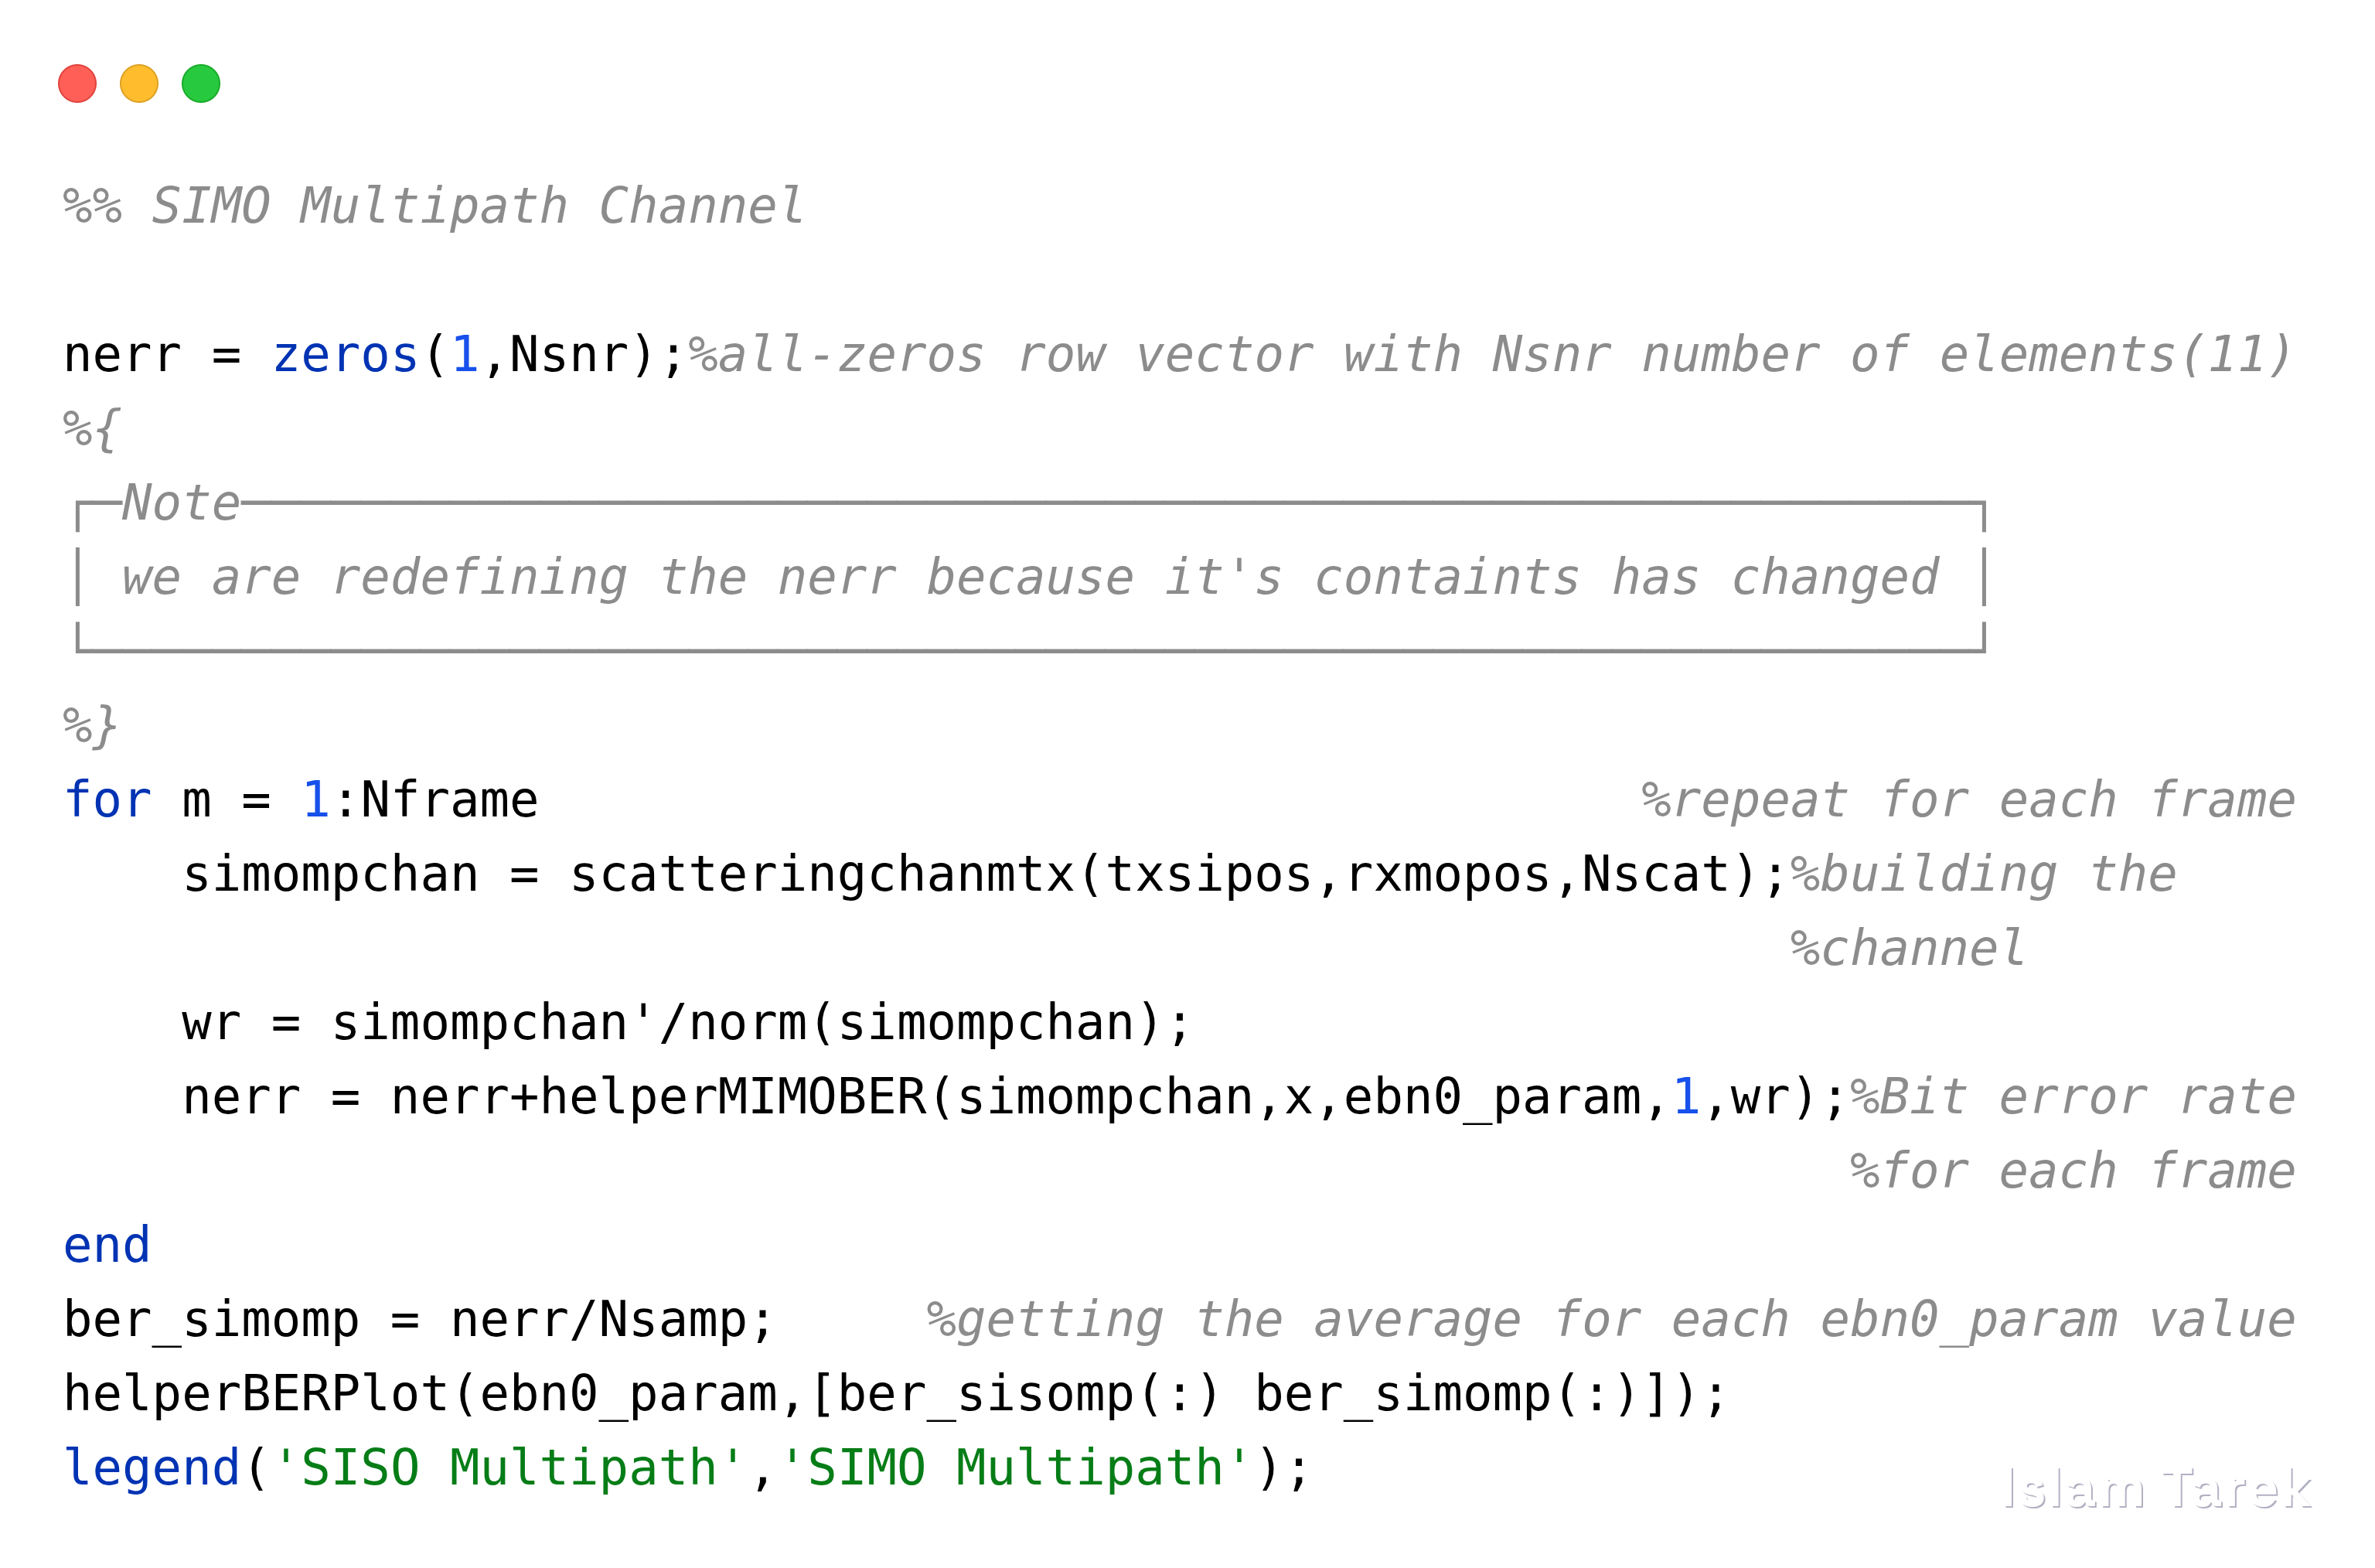
\includegraphics[width=0.7\linewidth]{figures/code7}
\end{figure}
\begin{figure}
	\centering
	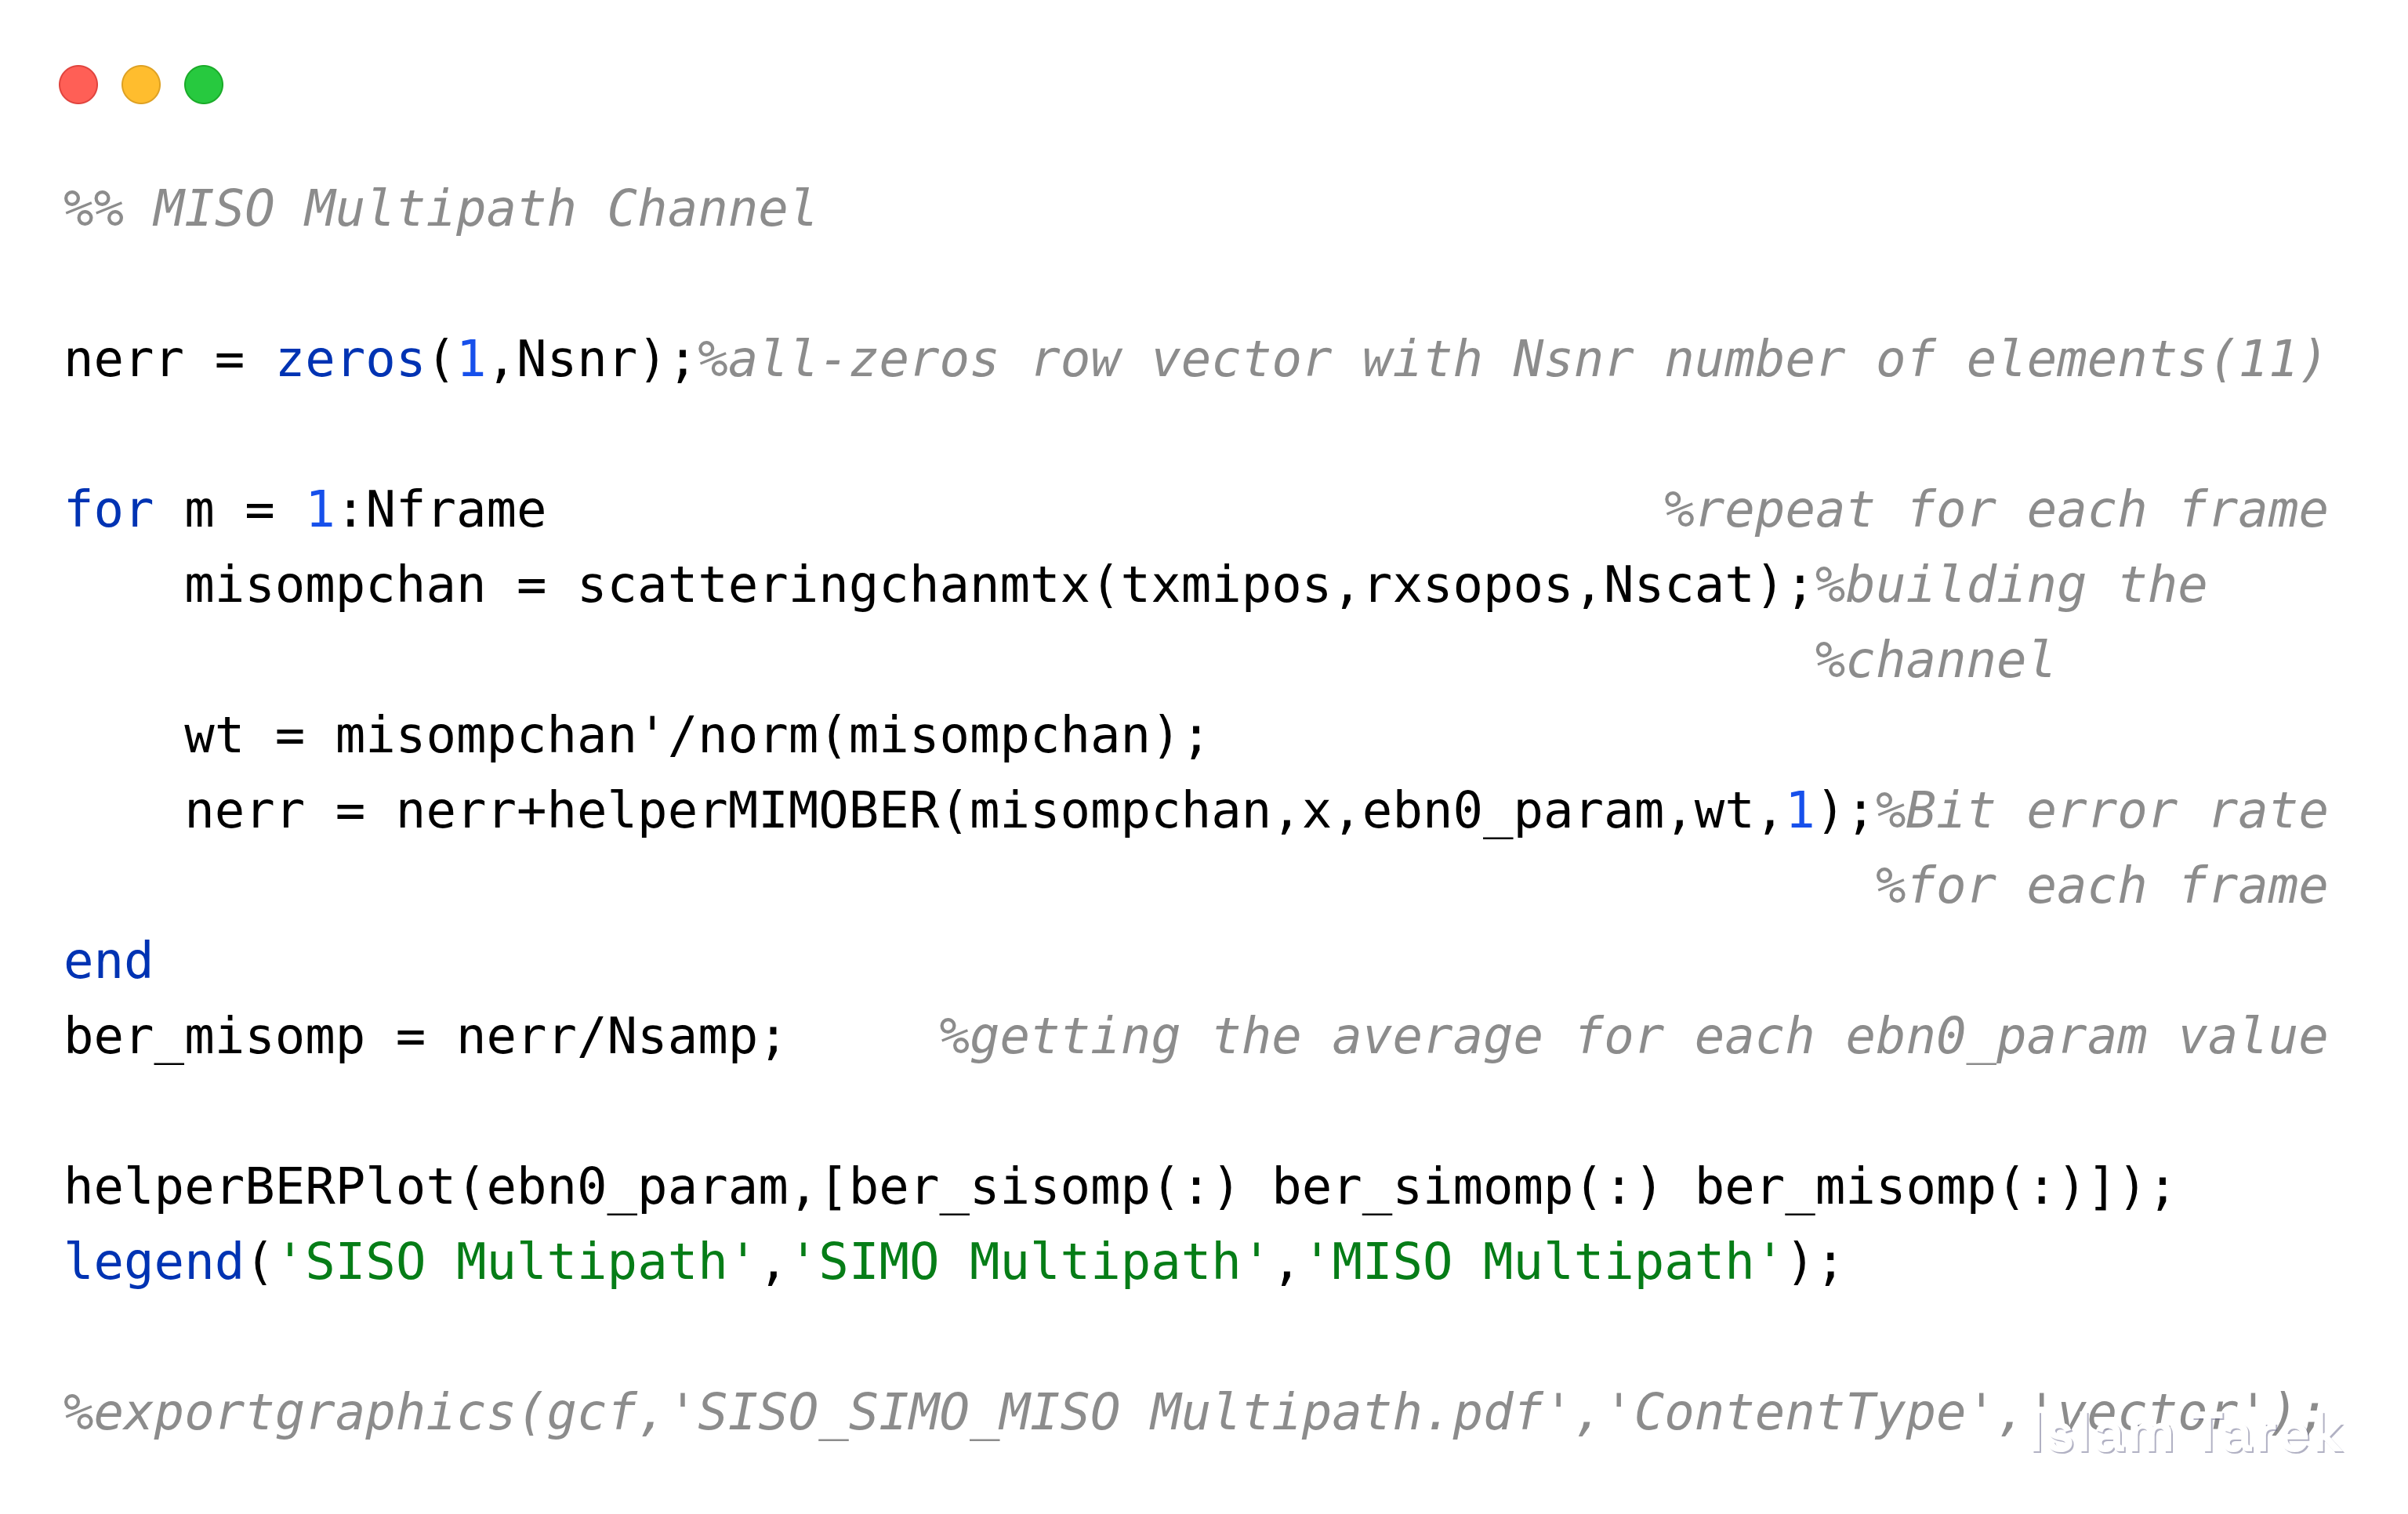
\includegraphics[width=0.7\linewidth]{figures/code8}
\end{figure}
\vfill
\restoregeometry